\setcounter{chapter}{3}

\chapter{The Interaction between Probabilistic Commitments and Knowledge}\label{cha:PCTLKC}


In this chapter\footnote{The results of this chapter have been published in the journal of Expert Systems with Applications \cite{Sultan2014b}.}, we
put forward a method for capturing and verifying the interactions between the concepts of knowledge and social commitments in probabilistic MASs. The proposed method allows us to figure out the impact of knowledge and social commitments on each other in the presence of uncertainty. To express the two concepts simultaneously in systems exhibiting probabilistic behavior, we define a new modal logic called the probabilistic logic of knowledge and commitments (PCTL$^{kc}$) which combines two existing probabilistic logics namely, the probabilistic logic of knowledge (PCTLK) \cite{Wan2012,Wan2013} and the probabilistic logic of commitments (PCTLC) that has been introduced in Chapter \ref{cha:PCTLC}. In the current chapter, MASs are modeled using a new version of interpreted systems that captures the probabilistic behavior and accounts for the communication between interacting components. Based on the proposed logic, we introduce a new model checking procedure to check the compliance of target systems against some desirable properties -- with respect to knowledge and commitments-- written in PCTL$^{kc}$. %and report some verification results.

\section{Introduction} \label{Introduction}

The rapid increase of using software agents and MASs nowadays has led to the increasing demand of finding principled techniques for modeling and verifying such systems. Generally, to build effective open MASs, several aspects which have direct influence on the efficiency and effectiveness of
the entire system must be taken into account \cite{Konur2013}.
Among other aspects, knowledge and social commitments are of a great
interest in MASs. Social commitments have been a vital approach in agent societies to capture the communication between interacting agents for more than a decade. On the other hand, knowledge has been addressed in distributed systems since 1960s \cite{Wan2013}. Recently, Al-Saqqar et al. \cite{Al-Saqqar2014a} have demonstrated that these two concepts are closely interacting with each other in various real life scenarios.

Despite the large amount of work that has been done to model and represent various aspect of probabilistic MAS, none of the existing approaches addresses the concepts of knowledge and social commitments simultaneously. In fact, the problem of reasoning about and verifying the interaction between knowledge and social commitments in the presence of uncertainty has not been investigated yet. Interpreted systems formalism \cite{Fagin1995}
and Partially Observable Markov Decision Processes POMDPs (a
variant of MDP) are the most prominent traditions in the area of
modeling and representing stochastic MASs. These models are used
to traditionally interpret some logics defined to specify and
reason about some given properties of MASs. On the one hand,
interpreted systems formalism provides a natural and yet efficient
way for modeling MASs at different levels of abstractions (i.e.,
local and global). It has been extended in \cite{Halpern2003} and
further in \cite{Wan2012,Wan2013} to capture the probabilistic
behavior of epistemic MASs. Recently, it has been extended in
\cite{Bentahar2012} and \cite{El-Menshawy2013a} to account for the
communication that occur between interacting parties in
conventional MASs. The distinct point of the extended versions of
this formalism is that knowledge and commitments can be captured
through the use of what is called accessibility relations. The
accessibility relation for knowledge denotes the existence of
equivalent states for a given agent. That is, states where the
agent cannot distinguish between being in which one of them. For
commitments, accessibility relations capture the existence of
communication channel between the communicating agents and the
transferring of information from the sender to the receiver. On
the other hand, POMDPs have been widely used to model the
uncertainty of knowledge and behavior for stochastic agents
\cite{Huang2011}. An important point of POMDPs is that there is no distinction drawn between actions taken to change the state of the world and actions taken to gain information \cite{Kaelbling1996}. This is important
because, in general, every action has both types of effect.
However, solving these models comes at a very high computational
cost \cite{Melo2011}. In this chapter, we aim to examine the use of interpreted systems formalism to capture not only knowledge and commitments
independently, but also the interactions (combinations) of the two
aspects in stochastic systems. We also intent to verify these
interactions by means of model checking.

In terms of computational logics, most current proposals address each of knowledge and commitments in MASs independently (see for example
\cite{Baldoni2010,Bentahar2012,Delgado2009,El-Menshawy2013a,Giordano2007,Halpern2003,Huang2011,Lomuscio2007,Pham2007,Wan2013}).
However, in so many real world settings, these two concepts need to
interact with each other in order to ensure rich modeling at local
(agent) and global (MAS) levels. Nevertheless, it is a challenge to guarantee the correctness of the system's behavior due to the complex nature of the autonomous and heterogenous agents, especially when they have probabilistic characteristics \cite{Song2012}.

Applying model checking techniques that were originally introduced
for standard logics, such as LTL \cite{Pnueli1977}, CTL
\cite{Emerson1990}, or PCTL \cite{Hansson1994}, to the
verification of the interaction between knowledge and social
commitments in presence of uncertainty is not straightforward as
non of these logics can capture and express the relationship
between knowledge and social commitments in probabilistic
settings. In this chapter, we introduce a model checking technique to address this open issue.

The motivation for the incorporation of knowledge and commitments
in a probabilistic logic is provided by the fact that these two
concepts not only have an impact on each other, but also their
interaction is crucial in various real scenarios. For instance, in
the field of mobile applications, which are complex in nature,
there exist situations when accounting for the interaction between
knowledge and commitments improves the output of such
applications. Let us consider a simple scenario where receiver and
sender agents share an agreement, in which the receiver agrees to
pay the sender in return of the delivery of a service he has
requested. This can be represented as a commitment, in which the
receiver will be committed to the sender to pay once the service
is made available for him. Now, if everything goes well and the
receiver successfully makes his payment, the sender has to know
that the payment is made so that he does not ask the receiver to
pay again. Moreover, the receiver (who made the payment) has to
know that he has fulfilled his commitment to avoid making multiple
payments, and so on. However, those interactions are stochastic.
For instance, the commitment to pay is not going to be surely
satisfied.


To effectively specify such properties in the face of uncertainty,
the need for a logical tool that can express probabilistic
knowledge and commitments simultaneously is indeed confirmed.
Rather than building a logic from scratch to address the
underlying aspects, we combine logics dealing with these two
individual units in a single logic. We advocate the approach of
combining existing logics because it ensures the preservation of
important properties of the logics being combined
\cite{Konur2013}. In particular, we use the independent join (or
fusion) technique \cite{Franceschet2004}. Given two logics $\mathbb{A}$ and $\mathbb{B}$, we combine them in a new logic $\mathds{A} \oplus \mathds{B}$ which extends the expressive power of each one. In our case, suppose $\mathds{A}$ addresses probabilistic epistemic properties of
agents and $\mathds{B}$ addresses the social aspects (i.e.,
probabilistic commitments and their fulfilments) between
interacting agents. Their combination should be able to not only
express epistemic and social properties, but also express the
interaction between the two concepts (i.e., express them in a
single formula). Once the new combined logic is defined, we use
the PRISM tool \cite{Kwiatkowska2002} as the formal verification tool to verify it after its reduction to PCTL, the probabilistic branching-time logic \cite{Hansson1994}.

The contributions of this chapter are threefold. First, we present a new probabilistic version of interpreted systems to model MASs using the dimensions of knowledge and social commitments. The developed version merges two extended versions of the original formalism of interpreted systems introduced by Fagin and his colleagues \cite{Fagin1995}. Those versions are introduced respectively by 1) Halpern \cite{Halpern2003} and extended later
by Wan et al. \cite{Wan2012,Wan2013} to capture the stochastic
behavior of the system; and 2) by Bentahar et al.
\cite{Bentahar2012} and El-Menshawy et al. \cite{El-Menshawy2013a}
to model the communication between interacting parties. Second, we
introduce a new logic called Probabilistic Logic of Knowledge and
Commitment (PCTL$^{kc}$) to be able to capture and reason about
the interaction between knowledge and social commitments. The
logic we define combines the Probabilistic Computation Tree Logic
of Knowledge PCTLK \cite{Wan2012,Wan2013} and the Probabilistic
Computation Tree Logic of Commitments PCTLC \cite{Sultan2013}.
PCTLK and PCTLC are, in turn, extensions of the Probabilistic
Computation Tree Logic PCTL \cite{Hansson1994} with an epistemic
modality for the knowledge and a social modality for the
commitments and their fulfilments respectively. Third, we
introduce a new model checking technique to verify the proposed
logic (PCTL$^{kc}$). The introduced technique is a reduction-based
in which the problem of model checking PCTL$^{kc}$ is transformed
into the problem of model checking an existing logic called PCTL.
To achieve this reduction, new rules have been laid down to
transform the models of PCTL$^{kc}$ to MDPs to be suitable for
the PRISM model checker. We also devise some other rules to reduce
each PCTL$^{kc}$ formula into PCTL formula. By so doing, we can
build on the existing PRISM model checker by automating our
translation to verify some given properties written originally in
our new logic PCTL$^{kc}$. Figure \ref{approach-cha4} gives an overview of the proposed approach.

\begin{figure}[h]
\begin{center}
\includegraphics [width=14cm, height=5cm]{chap4/img/approach-cha4.eps}
  \caption{An approach for the interaction between knowledge and commitments}
\label{approach-cha4}
\end{center}
\end{figure}


The work presented in this chapter represents a new trend in the direction of capturing interactions between various aspects in MASs. It can be
seen as a first attempt to combine the notions of probability,
knowledge, and commitments in a single tool giving a new
expressive power ---in terms of expressing the individual aspects
as well as their combinations in the presence of uncertainty---,
and is therefore subject to new intuitions.



\section{The Probabilistic Logic of Knowledge and Commitment (PCTL$^{kc})$} \label{sec:PCTLKC-logic}

In this section, we introduce our new probabilistic logic of knowledge and commitment (PCTL$^{kc})$. The modal logic we introduce can express knowledge and social commitments simultaneously in the presence of uncertainty. It combines two existing probabilistic logics namely, the probabilistic logic of knowledge PCTLK \cite{Wan2012,Wan2013} and the probabilistic logic of commitments PCTLC \cite{Sultan2014a,Sultan2013}. We first present the syntax of our new logic, and then we define its semantics. We also define a new version of the probabilistic interpreted systems formalism over which the semantics of PCTL$^{kc}$ can be interpreted.


As we said earlier, the new logic PCTL$^{kc}$ contains a knowledge modality that doesn't exist in the logic defined previously in Chapter \ref{cha:PCTLC}. Therefore, we need first to define the model of PCTL$^{kc}$. In fact, the PCTL$^{kc}$ model is generated from an extended version of probabilistic interpreted systems \cite{Halpern2003,Wan2013} enriched by the social accessibility relations introduced in \cite{Bentahar2012,El-Menshawy2013a} as discussed in Chapter \ref{cha:background}.


\begin{definition}[Models]\label{def:models-pctlkc}

Given a set of atomic propositions $\Phi_p = (p,q,r, \ldots)$ and a set of agents $\texttt{Agt}=\{1,\ldots,n\}$,  the model $\mathfrak{M_2}=(S,\textbf{P},I,\sim_1, \ldots
,\sim_n,\{\sim_{i \rightarrow j}\}_{{(i,j)}\in \texttt{Agt}^2},\nu)$ is a tuple where:
%
\begin{itemize}
\item  $S \subseteq L_1 \times \ldots \times L_n$ is a countable
set of all reachable global states for the system. A state $s$ is
reachable iff there exists a sequence of transitions from an
initial state to $s$ in which the probability of each transition
is greater than $0$.

\item  $I \in S$ is an initial global state for the system.


\item  $\textbf{P}:S\times S\rightarrow [0,1]$ is a total
transition probability function defined as $\textbf{P}(s,
s')=\tau(s,a^{s \rightarrow s'}, s')$ iff there exists a joint
action $a=(a_1,\ldots,a_n) \in ACT$ such that\\
 $\sum_{i \in \texttt{Agt}} \tau_i(l_i(s),a^{l_i(s)\rightarrow l_i(s')},l_i(s')) > 0$ and $\sum_{s' \in S} \textbf{P}(s,s') =1$
for all $s \in S$.

\item  $\sim_i \subseteq S \times S$ is the epistemic
  accessibility relation for the agent $i$, such that for two global states $s$ and $s'$, we have: $s \sim_i s'$ iff
  $l_i(s)=l_i(s')$.

\item For each pair $(i,j) \in \texttt{Agt}^2$,
$\sim_{i\rightarrow j} \subseteq S \times S$ is a serial social
accessibility relation. $s \sim_{i\rightarrow j} s'$ is defined by
the following conditions:
      %
  \begin{enumerate}
       \item $l_i(s)=l_i(s')$.
       \item $Var_i \cap Var_j \neq \emptyset$ such that $\forall x \in Var_i \cap Var_j$ we have $l^{x}_i(s)\!=\!l^{x}_j(s')$.
       \item $\forall y \in Var_j\!-\! Var_i$ we have $l^{y}_j(s)\!=\!l^{y}_j(s')$.
  \end{enumerate}
       %
  \item  $\nu : S\rightarrow 2^{\Phi_p}$ is a function valuating states with atomic propositions.
\end{itemize}
\end{definition}
%



The difference between our new model $\mathfrak{M_2}$ and the model $\mathfrak{M_1}$ that has been proposed in Chapter \ref{cha:PCTLC} is that $\mathfrak{M_2}$ has the ability to model agents' knowledge in the system --in addition to modeling the commitment-based communication among interacting parties-- thanks to the epistemic accessibility relations that are integrated in the model. Technically, $\mathfrak{M_2}$ in an extended version of $\mathfrak{M_1}$ with epistemic accessibility relations. Computation paths of $\mathfrak{M_2}$ and probability space are defined as in Chapter \ref{cha:PCTLC}. %(Section \ref{sec: semantics of PCTLC}).



\subsection{Syntax of PCTL$^{kc}$} \label{sec:syntax-PCTLKC}
The logic we introduce in this section can be seen as an extension to the logic presented in Chapter \ref{cha:PCTLC} by adding an epistemic operator to PCTLC \cite{Sultan2014a,Sultan2013}. The resulting logic, i.e., PCTL$^{kc}$, will have the power to not only express the individual aspects of knowledge and social commitments in independent formulae, but also express combinations of the two concepts in the same formulae.

\begin{definition}[Syntax]\label{def:PCTLKC syntax}
Given a set of atomic propositions $\Phi_p$. Let $\verb"Agt"=\{1, \dots, n\}$ be a set of agents. The PCTL$^{kc}$ formulae are defined by the following BNF grammar:
%
\begin{align*}
    \varphi & ::= p~|~\neg \varphi~|~\varphi \vee \varphi~|~\mathcal{K}~|~\mathcal{C}~|~ \mathbb{P}_{\bowtie k} (\psi)~|~\mathbb{P}_{\bowtie k}(\mathcal{K})|~\mathbb{P}_{\bowtie k}(\mathcal{C})\\
    \psi & ::=\bigcirc \varphi ~ | ~ \varphi ~U~ \varphi~|~ \varphi~ U^{\leq m} ~ \varphi \\
    \mathcal{K} & ::= K_i \varphi \\
    \mathcal{C} & ::= C_{i\rightarrow j}\varphi ~| ~ Fu(C_{i\rightarrow j}\varphi)
\end{align*}
%
where $p\in\Phi_p$ is an atomic proposition and $\mathbb{P}_{\bowtie
k}$ is a probabilistic operator where $\bowtie \in\{<,\leq,>,\ge\}$ and $k\in [0,1]$ is a probability bound or threshold. $m \in\mathbb{N}^+ $ is a positive integer number reflecting the maximum number of transitions needed to reach a certain state. $\varphi$ and $\psi$ are state and path formulae interpreted over the states and paths of $\mathfrak{M_2}$ respectively. The Boolean connectives $\neg$ and $\vee$ are defined in the usual
way. Formulae $\mathcal{K}$ are state formulae called knowledge (epistemic) formulae and used to express the epistemic properties through the K$_i$ operator which stands for agent i knows. Formulae $\mathcal{C}$, called social formulae, are special state formulae in PCTL$^{kc}$ that can express social properties using the modal connectives $C_{i\rightarrow j}$ and $Fu(C_{i\rightarrow j})$ standing for ``commitment'' and ``fulfillment of commitment'' respectively. $\bigcirc, U$ and $U^{\leq m}$ stand for ``next time'', ``until'' and ``bounded until'' path modal connectives
respectively.

\end{definition}



\subsection{Semantics of PCTL$^{kc}$} \label{def:semantics-PCTLKC}

Given a model $\mathfrak{M_2}=(S,\textbf{P},I,\sim_1, \ldots
,\sim_n,\{\sim_{i \rightarrow j}\}_{{(i,j)}\in \texttt{Agt}^2},\nu)$, then $(\mathfrak{M_2},s) \models \varphi$ states that ``a state $s$ in the model $\mathfrak{M_2}$ satisfies a state formula $\varphi$, $(\mathfrak{M_2},\pi) \models \psi$ means that ``a path $\pi$ in the model $\mathfrak{M_2}$ satisfies a path formula $\psi$, and
$(\mathfrak{M_2},s) \models \mathbb{P}_{\bowtie k}(\psi)$ means that
``a state $s$ in $\mathfrak{M_2}$ satisfies $\mathbb{P}_{\bowtie k}(\psi)$ if the probability of taking a path from $s$ that satisfies $\psi$ is in the interval specified by $\bowtie k$''. When the model $\mathfrak{M_2}$ is clear from the context, we simply write the satisfaction relation $\models$ as follows: $s \models \varphi$ and $\pi \models \psi$. Furthermore,
for a given pair $(i,j)\in \texttt{Agt}^2$ of agents, we denote
the number of socially accessible states $s'$ from a given state $s$ such
that $s\sim_{i\rightarrow j}s'$ by $|s\sim_{i\rightarrow j}s'|$.
We also denote the number of epistemically accessible states $s'$ from a given state $s$ such that $s\sim_i s'$ by $|s\sim_i s'|$.

Finally, we define $|s\models \varphi|$ as follows:

\begin{center}
$|s\models \varphi|=
\begin{cases}
1,~~~\textrm{if}~ s\models\varphi\\
0,~~~\textrm{otherwise.}
\end{cases}$
\end{center}

\begin{definition}[\textbf{Satisfaction}]\label{def:semantics-pctlkc} Satisfaction of a PCTL$^{kc}$ formula in the model $\mathfrak{M_2}$ is recursively defined as follows:

%\noindent In what follows, we define the semantics of PCTL$^{kc}$ formulae.

\noindent $s\models p~~~~~~~~~~~~~~\emph{iff}~~p\in \nu(s);\\
s\models \varphi_1 \vee \varphi_2 ~~~~~~\emph{iff}~~s\models \varphi_1~\textrm{or}~s \models \varphi_2; \\
s\models \neg \varphi~~~~~~~~~~~\emph{iff}~~s \nvDash \varphi;\\
s\models K_i \varphi  ~~~~~~~~~~ \emph{iff}~~ \forall s'\in S ~ \textrm{s.t.} ~~ s \sim_i s'  \ \textrm{we~have}~ s'\models \varphi; \\
s\models C_{i\rightarrow j}\varphi~~~~~~~~\emph{iff} ~~\forall s' \in S~\textrm{s.t.}~s \sim_{i \rightarrow j}s', \textrm{we~have}~s' \models \varphi;\\
s\models Fu(C_{i\rightarrow j}\varphi) ~~\emph{iff} ~~\exists s' \in S~\textrm{s.t.}~s' \sim_{i \rightarrow j}s ~ \textrm{and}~s' \models C_{i\rightarrow j}\varphi;$


\noindent $\pi \models \bigcirc \varphi~~~~~~~~~~~\emph{iff}~~\pi(1) \models \varphi; \\
\pi \models \varphi_1~U^{\leq m}~\varphi_2~~\emph{iff}~~\exists k \leq m~~\textrm{s.t.}~~ \pi(k) \models \varphi_2 ~\textrm{and}~\forall i < k, \pi(i) \models \varphi_1;\\
\pi \models \varphi_1 ~U~\varphi_2~~~~~~\emph{iff}~~\exists m \geq 0~~\textrm{s.t.}~~\pi \models \varphi_1~U^{\leq m}~\varphi_2;$



\noindent $s \models \mathbb{P}_{\bowtie k} (\psi)~~~~~~~~\emph{iff}~~Prob_s(\psi)\bowtie k$ where: $Prob_s(\psi)=Prob_s\{\pi \in \Pi(s)~|~\pi\models
\psi\};$

%\begin{itemize}
\noindent For a probabilistic operator working on an epistemic formula, where the set of all accessible states from $s$ is our sample space and the set of events $\mathrm{F}$ is the set of states accessible from $s$ and satisfy the formula:

\begin{tabbing}
$s\models \mathbb{P}_{\bowtie k}(K_i\varphi) $
    \ \ \ \ \ \= \emph{iff} \ $Prob(s \models K_i\varphi)$ $\bowtie k$ where: $Prob(s\models K_i\varphi)=\frac{\sum_{s \sim_i s'}|s'\models \varphi| }{|s \sim_i s'|};$

\end{tabbing}


\noindent For a probabilistic operator working over a commitment formula,
where the set of all accessible states from $s$ is our sample space and the set of events $\mathrm{F}$ is the set of states satisfying the formula: %and assuming that the probabilities of accessible states from state $s$ are equally distributed:


\noindent  $s\models \mathbb{P}_{\bowtie k}(C_{i\rightarrow j}\varphi)$
   ~\emph{iff}  $Prob(s \models C_{i\rightarrow j}\varphi) \bowtie \!k$ where: $Prob(s\models C_{i\rightarrow j}\varphi)=\frac{\sum_{s \sim_{i \rightarrow j}s'}|s'\models \varphi| }{|s \sim_{i \rightarrow j}s'| };$


\noindent For a probabilistic operator working over a fulfilment formula,
 assuming that accessible states are also reachable:

\noindent $s\models \mathbb{P}_{\bowtie k}(Fu(C_{i\rightarrow j}\varphi))$
    ~~ \emph{iff}~ $Prob(s \models Fu(C_{i\rightarrow j}\varphi)) \bowtie k;$ where:
%\vspace{-0.4cm}
\begin{align*}
& Prob(s\models Fu(C_{i\rightarrow j}\varphi))\ = Prob_s\{\pi \in \Pi(s') ~|~ s' \sim_{i \rightarrow j}s ~~\textrm{and}~~ \pi = s' \ldots s ~~\textrm{and}~~ s' \models C_{i\rightarrow j}\varphi\}
\end{align*}


%\end{itemize}
\end{definition}

The probabilistic knowledge is computed in such a way to reflect the indistinguishability property of the epistemic accessibility relations. Therefore, the probability is computed based on the number of accessible states satisfying the content of the knowledge over the number of equivalent states, as all the states are equally accessible. Probabilistic commitment is also computed based on the number of accessible states that satisfy the
content over the whole number of accessible states, which demonstrates the uncertainty of the agent over the accessible states, so that over the commitment. Probabilistic fulfillment, however, is computed using the probabilistic transitions of the path linking the commitment state to the fulfillment state. The following proposition is straightforward from the semantics:

\begin{proposition} \label{proposition-PCTLKC}~\\
If $(\mathfrak{M_2},s)\models \mathbb{P}_{\leq0} (Fu(C_{i \rightarrow
j}\varphi))$ and $(\mathfrak{M_2},s)\models Fu(C_{i \rightarrow
j}\varphi)$, then $s$ is not reachable from the commitment state.
\end{proposition}


\begin{theorem} \label{thm: Ki equivalence} \ \ \ \ {Epistemic Equivalences}

    \begin{enumerate}
        \item $(\mathfrak{M_2},s)\models \mathbb{P}_{\geq1}(K_i\phi)$  ~~~~~iff~~  $(\mathfrak{M_2},s) \models K_i\phi$
        \item $(\mathfrak{M_2},s)\models \mathbb{P}_{\leq 0}(K_i\phi)$   ~~~~~iff~~  $(\mathfrak{M_2},s)\models K_i \neg \phi$
        \item $(\mathfrak{M_2},s)\models \mathbb{P}_{]0,1[}(K_i~\phi)$  ~~~iff~~   $(\mathfrak{M_2},s)\models \neg K_i\neg\phi \wedge \neg K_i\phi$

    \end{enumerate}

\end{theorem}


\begin{proof} \hspace{-0.9cm}

\begin{itemize}
\item First equivalence. ~\\
    $``\Rightarrow"$. Assume $s\models \mathbb{P}_{\geq1} (K_i\varphi)$.
    By the semantics of PCTL$^{kc}$, it follows that $Prob(s\models K_i\varphi)\geq1$.
    Therefore, $\frac{\sum_{s\sim_i s'}|s'\models \varphi| }{|s\sim_i s'|}\geq1$. This means $\forall s'\in S$ such that $s\sim_i s'$, we have
    $s'\models \varphi$ (as $\sim_i$ is reflexive, so $s'$ could be $s$ itself). Thus, $s \models K_i \varphi$. \\
    $``\Leftarrow"$. Assume $s\models K_i\varphi$. By the PCTL$^{kc}$ semantics, it follows that for all $s'\in S$ such that $s\sim_i s'$,
    we have $s'\models \varphi$ (i.e. all accessible states from $s$ satisfy $\varphi$).
    Consequently, $\sum_{s\sim_i s'}|s'\models \varphi| = |s\sim_i s'|$.
    Therefore, $\frac{\sum_{s\sim_i s'}|s'\models \varphi| }{|s\sim_i s'|}\geq1$ and hence $s\models \mathbb{P}_{\geq1} (K_i\varphi)$.

\item Second equivalence. ~\\
    $``\Rightarrow"$. Assume $s\models \mathbb{P}_{\leq0} (K_i\varphi)$.
    By the PCTL$^{kc}$ semantics, it follows that $Prob(s\models K_i\varphi)\leq0$.
    Thus, $\frac{\sum_{s\sim_i s'}|s'\models \varphi|}{|s\sim_i s'|}\leq0$. Since $\sim_i$ is reflexive, so the set of the accessible states from $s$ is not empty, therefore $\sum_{s\sim_i s'}|s'\models \varphi|$ must be 0 (i.e. $\varphi$ is not true in any of the accessible states). Consequently, for all $s'\in S$ such that $s\sim_i s'$, we have $s'\nvDash \varphi$, which means $s'\vDash \neg \varphi$. Hence, $s\models K_i \neg \varphi$.~\\
%
    $``\Leftarrow"$. Assume $s\models K_i\neg \varphi$. By the PCTL$^{kc}$ semantics, it follows that $\forall s'\in S$ such that
    $s\sim_i s'$, we have $s'\nvDash \varphi$. Since the set of the accessible states from $s$ is not empty, then $\frac{\sum_{s\sim_i s'}|s'\models \varphi| }{|s\sim_i s'|}\leq0$.
    Hence, $s\models \mathbb{P}_{\leq0} (K_i\varphi)$.

\item Third equivalence. ~\\
    $``\Rightarrow"$. Assume $s\models \mathbb{P}_{]0,1[} K_i\varphi)$. By the PCTL$^{kc}$ semantics, it follows that $0< Prob(s\models K_i\varphi)<1$. Thus, $0<\frac{\sum_{s\sim_i s'}|s'\models \varphi| }{|s \sim_i s'|}<1$.
    This means that it would never be the case that $\sum_{s\sim_i s'}|s'\models \varphi| = |s\sim_i s'|$ nor $\sum_{s\sim_i s'}|s'\models \varphi| = 0$. Consequently, there exist some $s', s'' \in S$ such that $s\sim_i s'$ and $s\sim_i s''$ and $s'\models \varphi$ and $s''\models \neg \varphi$. Hence, it is impossible to have $\overline{s}\models \neg\varphi$ or $\overline{s}\models \varphi$ for all $\overline{s}\in S$ such that $s\sim_i \overline{s}$. Consequently, $s\nvDash  K_i\neg\varphi$ and $s\nvDash K_i\varphi$. Hence $s\models \neg K_i\neg\varphi$ and $s\models \neg K_i\varphi$. ~\\
    %
    $``\Leftarrow"$. Assume $s\models \neg K_i\varphi$. By the PCTL$^{kc}$ semantics, it follows that there exists $s'\in S$ such that $s\sim_i s'$ and $s'\models \neg \varphi$. Consequently, it would never be the case that for all $s'\in S$ such that $s\sim_i s'$ we have $s'\models \varphi$. Therefore, $1>\frac{\sum_{s\sim_i s'}|s'\models \varphi| }{|s\sim_i s'|}$. Now assume $s\models \neg K_i\neg \varphi$. Therefore, $\sum_{s\sim_i s'}|s'\models \varphi| = 0$ would never be the case as some accessible states should satisfy $\varphi$. Consequently, $\frac{\sum_{s\sim_i s'}|s'\models \varphi| }{|s\sim_i s'|}>0$. Thus, $0<\frac{\sum_{s\sim_i s'}|s'\models \varphi| }{|s \sim_i s'|}<1$. Hence, $s\models \mathbb{P}_{]0,1[} (K_i\varphi)$.
\end{itemize}
\end{proof}

\vspace{0.9cm}
\begin{theorem}\label{Commitment-Equivelances}{Commitment Equivalences} ~

\begin{enumerate}
\item $(\mathfrak{M_2},s)\models \mathbb{P}_{\geq1} (C_{i \rightarrow
j}\varphi)$ ~~~iff~~ $(\mathfrak{M_2},s)\models C_{i \rightarrow
j}\varphi$

\item $(\mathfrak{M_2},s)\models \mathbb{P}_{\leq0} (C_{i \rightarrow
j}\varphi)$ ~~~iff~~ $(\mathfrak{M_2},s)\models C_{i \rightarrow
j}\neg \varphi$

\item $(\mathfrak{M_2},s)\models \mathbb{P}_{]0,1[} (C_{i \rightarrow
j}\varphi)$ ~~iff~~ $(\mathfrak{M_2},s)\models \neg C_{i
\rightarrow j}\neg\varphi \wedge \neg C_{i \rightarrow j}\varphi$

\end{enumerate}

\end{theorem}
%\vspace{1cm}
\begin{proof}\hspace{-0.9cm}


\begin{itemize}
\item First equivalence. ~\\
    $``\Rightarrow"$. Assume $s\models \mathbb{P}_{\geq1} (C_{i \rightarrow j}\varphi)$.
    By the PCTL$^{kc}$ semantics, it follows that $Prob(s\models C_{i\rightarrow j}\varphi)\geq1$.
    Thus,  $\frac{\sum_{s\sim_{i \rightarrow j}s'}|s'\models \varphi| }{|s\sim_{i \rightarrow j}s'|}\geq1$.
    This means that for all $s'\in S$ such that $s\sim_{i \rightarrow j}s'$, we have
    $s'\models \varphi$, and hence $s \models C_{i\rightarrow j}\varphi$. \\
    $``\Leftarrow"$. Assume $s\models C_{i \rightarrow j}\varphi$. By the
    PCTL$^{kc}$ semantics, it follows that for all $s'\in S$ such that $s\sim_{i \rightarrow j}s'$,
    we have $s'\models \varphi$ (i.e. all accessible states from $s$ satisfy $\varphi$).
    Consequently, $\sum_{s\sim_{i \rightarrow j}s'}|s'\models \varphi| = |s\sim_{i \rightarrow j}s'|$.
    Therefore, $\frac{\sum_{s\sim_{i \rightarrow j}s'}|s'\models \varphi| }{|s\sim_{i \rightarrow j}s'|}\geq1$
    and hence, $s\models \mathbb{P}_{\geq1} (C_{i \rightarrow j}\varphi)$.

\item Second equivalence. ~\\
    $``\Rightarrow"$. Assume $s\models \mathbb{P}_{\leq0} (C_{i \rightarrow j}\varphi)$.
    By the PCTL$^{kc}$ semantics, it follows that $Prob(s\models C_{i\rightarrow j}\varphi)\leq0$.
    Thus, $\frac{\sum_{s\sim_{i \rightarrow j}s'}|s'\models \varphi|}{|s\sim_{i \rightarrow j}s'|}\leq0$.
    Since the set of the accessible states from $s$ is not empty, then $\sum_{s\sim_{i \rightarrow j}s'}|s'\models \varphi|$
    must be 0 (i.e. $\varphi$ is not true in any of the accessible states). Consequently, for all $s'\in S$
    such that $s\sim_{i \rightarrow j}s'$, we have $s'\nvDash \varphi$, which means $s'\vDash \neg \varphi$.
     Hence, $s\models C_{i\rightarrow j}\neg \varphi$.~\\
%
    $``\Leftarrow"$. Assume $s\models C_{i \rightarrow j}\neg \varphi$. By the PCTL$^{kc}$ semantics,
    it follows that for all $s'\in S$ such that
    $s\sim_{i \rightarrow j}s'$, we have $s'\nvDash \varphi$. Since the set of the accessible states from $s$ is not empty,
    then $\frac{\sum_{s\sim_{i \rightarrow j}s'}|s'\models \varphi| }{|s\sim_{i \rightarrow j}s'|}\leq0$.
    Hence, $s\models \mathbb{P}_{\leq0} (C_{i \rightarrow j}\varphi)$.

\item Third equivalence. ~\\
    $``\Rightarrow"$. Assume $s\models \mathbb{P}_{]0,1[} (C_{i \rightarrow j}\varphi)$. By the PCTL$^{kc}$ semantics,
    it follows that $0< Prob(s\models C_{i\rightarrow j}\varphi)<1$. Thus,
    $0<\frac{\sum_{s\sim_{i \rightarrow j}s'}|s'\models \varphi| }{|s \sim_{i \rightarrow j}s'|}<1$.
    This means that it would never be the case that $\sum_{s\sim_{i \rightarrow j}s'}|s'\models \varphi| = |s\sim_{i \rightarrow j}s'|$
    nor $\sum_{s\sim_{i \rightarrow j}s'}|s'\models \varphi| = 0$. Consequently, there exist some $s', s'' \in S$
    such that $s\sim_{i \rightarrow j}s'$ and $s\sim_{i \rightarrow j}s''$ and $s'\models \varphi$ and $s''\models \neg \varphi$.
    Hence, it is impossible to have
    $\overline{s}\models \neg\varphi$ or $\overline{s}\models \varphi$ for all $\overline{s}\in S$
    such that $s\sim_{i \rightarrow j}\overline{s}$. Consequently,
    $s\nvDash  C_{i \rightarrow j}\neg\varphi$ and $s\nvDash  C_{i \rightarrow
    j}\varphi$. Hence $s\models \neg C_{i \rightarrow j}\neg\varphi$ and $s\models \neg C_{i \rightarrow j}\varphi$. ~\\
    %
    $``\Leftarrow"$. Assume $s\models \neg C_{i \rightarrow j}\varphi$. By the PCTL$^{kc}$ semantics,
    it follows that there exists $s'\in S$ such that $s\sim_{i \rightarrow j}s'$ and $s'\models \neg \varphi$.
    Consequently, it would never be the case that $s'\models \varphi$ for all $s'\in S$
    such that $s\sim_{i \rightarrow j}s'$. Therefore,
    $1>\frac{\sum_{s\sim_{i \rightarrow j}s'}|s'\models \varphi| }{|s\sim_{i \rightarrow j}s'|}$.
    Now assume $s\models \neg C_{i \rightarrow j}\neg \varphi$. Therefore, $\sum_{s\sim_{i \rightarrow j}s'}|s'\models \varphi| = 0$
    would never be he case as some accessible states should satisfy $\varphi$. Consequently,
    $\frac{\sum_{s\sim_{i \rightarrow j}s'}|s'\models \varphi| }{|s\sim_{i \rightarrow j}s'|}>0$.
    Thus, $0<\frac{\sum_{s\sim_{i \rightarrow j}s'}|s'\models \varphi| }{|s \sim_{i \rightarrow j}s'|}<1$.
    Thus, $s\models \mathbb{P}_{]0,1[} (C_{i \rightarrow
    j}\varphi)$.
\end{itemize}

\end{proof}

%%%%%%%%%%%%%%%%%%%%%%%%%%%%%%%%%%

\begin{theorem}\label{Fulfiilemt-Equivelances} {Fulfillment Equivalences}~

\begin{enumerate}
\item $(\mathfrak{M_2},s)\models \mathbb{P}_{>0} (Fu(C_{i \rightarrow
j}\varphi))$ iff $(\mathfrak{M_2},s)\models Fu(C_{i \rightarrow
j}\varphi)$ and $s$ is reachable from the commitment state.

\item $(\mathfrak{M_2},s)\models \mathbb{P}_{\leq0} (Fu(C_{i \rightarrow
j}\varphi))$ iff $(\mathfrak{M_2},s)\models \neg Fu(C_{i \rightarrow
j}\varphi)$ or $s$ is not reachable from the commitment state.

\end{enumerate}

\end{theorem}

\begin{proof} \hspace{0.5cm} \\
The proofs of these equivalences are direct from Proposition
\ref{proposition-PCTLKC} and the above semantics.

 \end{proof}

\section{Model Checking PCTL$^{kc}$ Using Reduction} \label{sec:model-checking-pctlkc}


In this section, we present our reduction technique to model checking PCTL$^{kc}$. Given a MAS represented as a probabilistic interpreted system $\mathfrak{M_2}$ and a desirable property $\varphi$ written in PCTL$^{kc}$, the problem of probabilistic model checking PCTL$^{kc}$ can be defined as: 1) establishing whether $(\mathfrak{M_2}, I)\models \varphi$,
i.e., if $I \in Sat(\varphi)$ where $Sat(\varphi)$=$\{s\in S ~~|~~
\mathfrak{M_2},s \models \varphi \}$ is the set of states satisfying
$\varphi$; 2) comparing the probability of satisfying $\varphi$
with a probability threshold $\bowtie k$, where
$Sat(\mathbb{P}_{\bowtie k}(\varphi))=\{s\in S ~|~
Prob_s(\varphi)\bowtie k \}$ ; or 3) computing the probability of
$\varphi$, $(\mathfrak{M_2}, s)\models \mathbb{P}_{=?} ~(\varphi)$.
Note that answers to the second and third queries can be: (1)
truth values, when the specification simply asks for a comparison
to a probability threshold; or (2) quantitative, returning the
actual probability.

Figure \ref{fig:reduction-process-PCTLKC} depicts the structure of our proposed reduction technique. The idea is to reduce the problem of probabilistic model checking PCTL$^{kc}$ to the problem of probabilistic model checking PCTL in order to use the PRISM model checker. Concretely, the proposed reduction technique consists of two processes. In the former one, we transform our model $\mathfrak{M_2}$ into an MDP model.
MDPs are the standard models for describing systems with probabilistic and nondeterministic behavior \cite{Rutten2004}. Then, we use the notion of adversary as in \cite{Kwiatkowska2003} to resolve the nondeterminism of the MDP. The resulting adversaries are basically DTMC models for which we can define a unique probability measure over paths. The obtained DTMC models will be the input of the PRISM model checker. In the latter process of the reduction technique, we transform PCTL$^{kc}$ formulae into PCTL formulae. This is basically achieved by constructing a set of rules that formally transforms the PCTL$^{kc}$ formulae into corresponding ones in PCTL.

\begin{figure}[h]
\centering
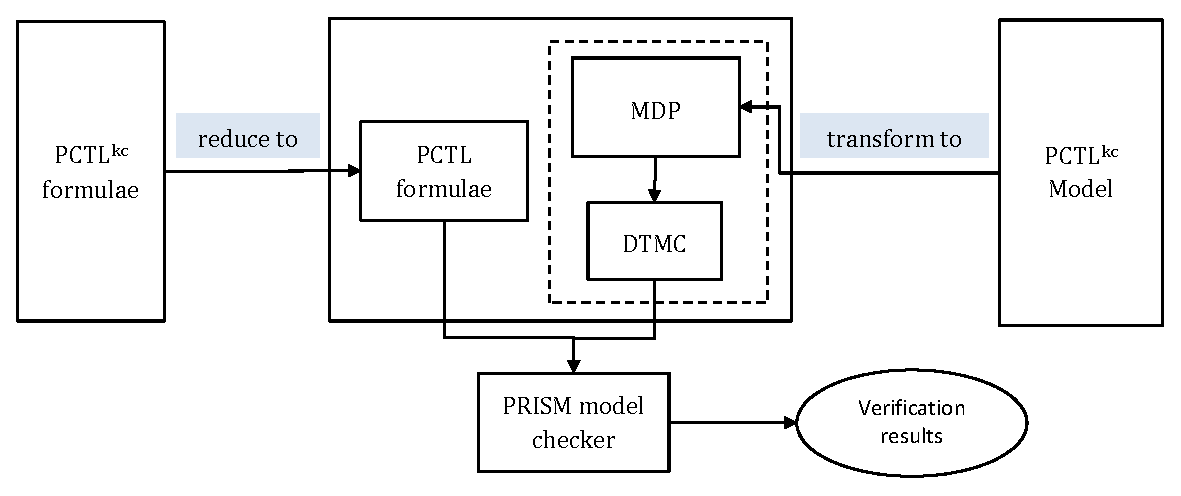
\includegraphics[width=14cm, height=7cm]{chap4/img/reduction-process-cha4.eps}
%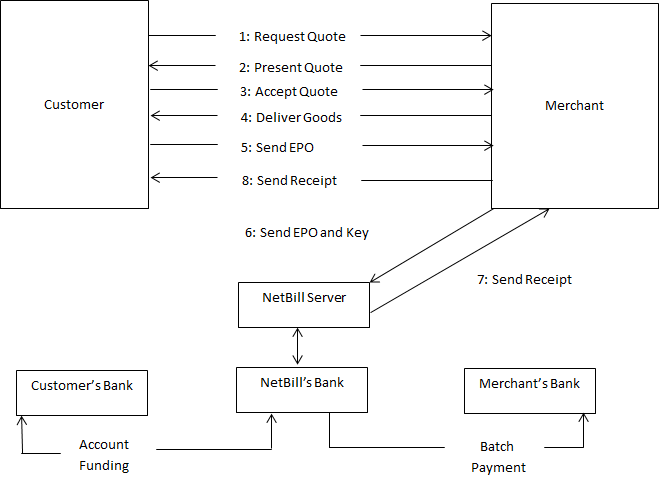
\includegraphics[scale=0.5]{figure1}
\caption{The proposed reduction technique of model checking PCTL$^{kc}$}
\label{fig:reduction-process-PCTLKC}
\end{figure}


In a nutshell, the proposed model checking procedure is as follows. Given $\mathfrak{M_2}=(S,\textbf{P},I,\sim_1, \ldots
,\sim_n,\{\sim_{i \rightarrow j}\}_{{(i,j)}\in \texttt{Agt}^2},\nu)$, and PCTL$^{kc}$ formula $\varphi$, we have to define an MDP model $\mathfrak{M'_2}$ = $\mathscr{F}(\mathfrak{M_2})$ and PCTL formula $\mathscr{F}(\varphi)$ using the transformation function $\mathscr{F}$ such that $\mathfrak{M_2} \models \varphi$ iff $\mathscr{F}(\mathfrak{M_2})\models \mathscr{F}(\varphi)$.


\begin{figure}[h]
\centering
\includegraphics[width=15cm, height=9cm]{chap4/img/relation-translation2.eps}
%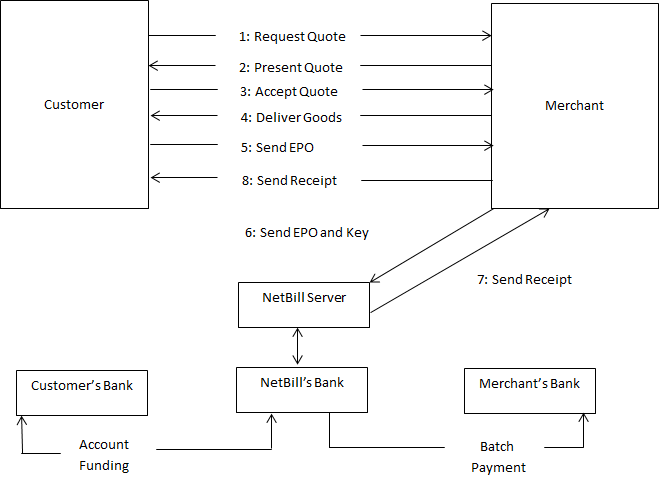
\includegraphics[scale=0.5]{figure1}
\caption{Translating relations in $\mathfrak{M_2}$ into labeled transitions in the MDP model} \label{fig:relation-translation-PCTLKC}
\end{figure}

\subsection{Transforming the Model $\mathfrak{M_2}$}

In order to transform our model $\mathfrak{M_2}=(S,\textbf{P},I,\sim_1, \ldots
,\sim_n,\{\sim_{i \rightarrow j}\}_{{(i,j)}\in \texttt{Agt}^2},\nu)$ into an MDP model $\mathfrak{M'_2}$ = $(\mathbb{S}, Act, \textsf{P}_t ,I_i, L)$, we need to define the set of actions $Act$. Therefore, one of the main steps that we perform in this transformation is to define the set $Act$. The idea is that, we translate different relations in $\mathfrak{M_2}$ into labeled transitions in $\mathfrak{M'_2}$. Labels (also called actions) are used to distinguish between different types of relations. Consequently, the three relations in $\mathfrak{M_2}$, namely transition relation, epistemic accessibility relation, and social accessibility relation are translated into labeled transitions in $\mathfrak{M'_2}$. Moreover, whenever we have a labeled transition representing a social accessibility relation we add the symmetric closure of it to interpret the fulfilment of the commitment. As depicted in Figure \ref{fig:relation-translation-PCTLKC} (assuming that $n$ is the number of agents, $1 \leq i \leq n$, and $1 \leq j \leq n$), actions $\delta, \alpha^i, \beta^{ij},$ and $\gamma^{ij}$ denote transitions defined, respectively, from the probabilistic transition relation $\textbf{P}$, the epistemic accessibility relation $\sim_i$ (to capture the semantics of knowledge), the social accessibility relation $\sim_{i \rightarrow j}$ (to capture the semantics of commitment), and the symmetric closure of the social accessibility relation (to capture the semantics of fulfilment).\\

The MDP model $\mathfrak{M'_2} = (\mathbb{S}, Act, \textsf{P}_t ,I_i, L)$ can now be defined as follows:


\begin{itemize}
\item $\mathbb{S}$=$S$; $I_i$=$I$; $L$=$\nu$.

\item $Act = \{\delta \} \cup \{\alpha^1, \alpha^2, \dots, \alpha^n\} \cup \{\beta^{11}, \beta^{12}, \dots, \beta^{nn}\} \cup \{\gamma^{11}, \gamma^{12}, \dots, \gamma^{nn}\}$ where $n$ is the number of agents.

\item We define $\textsf{P}_t$ as the union of the transitions labeled with $\delta$ (i.e., the probabilistic transitions of $\textbf{P}$) with the probabilistic transitions labeled with $\alpha^i$, probabilistic transitions labeled with $\beta^{ij}$, and probabilistic transitions labeled with $\gamma^{ij}$. The probabilities of transitions labeled with $\delta$ are not manipulated but rather inherited from the probabilistic transition function $\textbf{P}$. However, for transitions labeled with $\alpha^i$ and emanating from the same state are given equal probabilities (i.e., equal distribution) which reflect the uncertainty of the agent over the accessible states, so that over the content of the knowledge. Meaning that, the probability of each transition annotated by $\alpha^i$ is equal to the probability of each other transition labeled with $\alpha^i$ emanating from the same state which is calculated by dividing one over the number of transitions labeled with $\alpha^i$. The probabilities of transitions labeled with $\beta^{ij}$ and $\gamma^{ij}$ are calculated in the same way. For states $s, s' \in \mathbb{S}$ and  action $\theta \in Act$, the function $\textsf{P}_t$ is defined as follows:
\begin{equation*}
    \textsf{P}_t(s, \theta , s' )=
\begin{cases}
    \textbf{P}(s, s'),   & \textit{if } \theta = \delta  \\
    \frac{1}{|s\sim_i s'|},   & \textit{if } \theta = \alpha^i\\
    \frac{1}{|s\sim_{i \rightarrow j} s'|},   & \textit{if } \theta = \beta^{ij}\\
    \frac{1}{|s'\sim_{i \rightarrow j} s|},   & \textit{if } \theta = \gamma^{ij}.
    \end{cases}
    \end{equation*}

\end{itemize}


The induced model of applying the adversary $\sigma$ over
$\mathfrak{M'_2}$ is a DTMC model. Specifically, four adversaries are defined; $\sigma_t$ over which temporal formulae are interpreted, $\sigma_e$ to capture epistemic formulae, $\sigma_c$ to capture commitment formulae, and $\sigma_f$ to capture fulfillment formulae. These adversaries are defined based on the following rules. To define $\sigma_t$, action $\delta$ is selected at every state in $\mathfrak{M'_2}$. For $\sigma_e$, action $\alpha^i$ has to be among the enabled actions at the knowledge state. Then, the adversary picks up $\alpha^i$ at that knowledge state and $\delta$ at every other state. Adversaries $\sigma_c$, and $\sigma_f$ are defined in the same way.

\subsection{Reducing PCTL$^{kc}$ Formulae into PCTL Formulae}

In this section, we introduce our reduction rules that translate PCTL$^{kc}$ formulae to PCTL formulae w.r.t given adversary $\sigma$. Given the adversary $\sigma_t$, the PCTL$^{kc}$ formulae are transformed
inductively into PCTL as follows:

$\mathscr{F}(p)=p$, if $p$ is an atomic proposition,

$\mathscr{F}(\neg \varphi)= \neg \mathscr{F} (\varphi)$,

$\mathscr{F}(\mathbb{P}_{\bowtie k}(\varphi \vee \psi))=\mathbb{P}_{\bowtie k}(\mathscr{F}(\varphi) \vee \mathscr{F}(\psi))$,

$\mathscr{F}(\mathbb{P}_{\bowtie k}\bigcirc \varphi)=\mathbb{P}_{\bowtie k} \bigcirc \mathscr{F}(\varphi)$,

$\mathscr{F}(\mathbb{P}_{\bowtie k}(\varphi~ U ~ \psi))=\mathbb{P}_{\bowtie k} (\mathscr{F}(\varphi) U \mathscr{F}(\psi))$,

$\mathscr{F}(\mathbb{P}_{\bowtie k}(\varphi~ U^{\leq m} ~ \psi))=\mathbb{P}_{\bowtie k} (\mathscr{F}(\varphi) U^{\leq m} \mathscr{F}(\psi))$,

Note that $\sigma_t$ is a DTMC model that is used to interpret only PCTL formulas. It cannot be used to capture the transformed formulas of knowledge and commitment as it ignores all relations except those labeled by $\delta$ (i.e., transition relations of $\textbf{P}$).

Given the adversary $\sigma_e$, the PCTL$^{kc}$ epistemic formula is transformed inductively into PCTL as follows:

$\mathscr{F}(K_i \varphi)= \mathbb{P}_{\geq 1}(\bigcirc \mathscr{F}(\varphi))$,

$\mathscr{F}(\mathbb{P}_{\bowtie k} K_i \varphi)= \mathbb{P}_{\bowtie k}(\mathbb{P}_{\geq 1}\bigcirc\mathscr{F}(\varphi))$,


As mentioned earlier, the adversary $\sigma_e$ is a DTMC model that captures only action $\alpha^i$ at the knowledge state and $\delta$ at all other states. Intuitively, transitions labeled with $\alpha^i$ represent epistemic accessibility relations and, in fact, epistemically accessible states from the knowledge state must satisfy $\varphi$. Back to Figure \ref{fig:relation-translation-PCTLKC} (b), it is readily seen that all next states to the knowledge state through transitions labeled with $\alpha^i$ satisfy $\mathscr{F}(\varphi)$. This explains why knowledge formula $K_i~\varphi$ is transformed to next operator followed by the transformation of the content of the knowledge $(i.e., \bigcirc \mathscr{F}(\varphi))$ in all paths emanating from the knowledge state.

Given the adversary $\sigma_c$, the PCTL$^{kc}$ commitment formula is
transformed inductively into PCTL as follows:

$\mathscr{F}(C_{i\rightarrow j}\varphi)= \mathbb{P}_{\geq 1}(\bigcirc \mathscr{F}(\varphi))$,

$\mathscr{F}(\mathbb{P}_{\bowtie k} C_{i\rightarrow j}\varphi)= \mathbb{P}_{\bowtie k}(\mathbb{P}_{\geq 1}\bigcirc\mathscr{F}(\varphi))$,

Similar to the case of knowledge formula, Figure \ref{fig:relation-translation-PCTLKC} (c) illustrates the intuitions behind transforming the commitment formula $C_{i\rightarrow j}\varphi$ to  $\bigcirc \mathscr{F}(\varphi)$ in all baths emerging from the commitment state.

Given the adversary $\sigma_f$, the PCTL$^{kc}$ fulfillment formula
is transformed inductively into PCTL as follows:

$\mathscr{F}(Fu(C_{i\rightarrow j}\varphi))= \mathbb{P}_{\geq 1}(\bigcirc \mathscr{F}(C_{i\rightarrow j}\varphi))= \mathbb{P}_{\geq 1}(\bigcirc\mathbb{P}_{\geq 1}(\bigcirc \mathscr{F}(\varphi)))$,

$\mathscr{F}(\mathbb{P}_{\bowtie k} Fu(C_{i\rightarrow j}\varphi))= \mathbb{P}_{\bowtie k} (\mathbb{P}_{\geq 1}\bigcirc\mathscr{F}(C_{i\rightarrow j}\varphi))= \mathbb{P}_{\bowtie k}(\mathbb{P}_{\geq 1}\bigcirc\mathbb{P}_{\geq 1}(\bigcirc \mathscr{F}(\varphi)))$.

Though the semantics of the fulfillment operator in PCTL$^{kc}$ requires the existence of a path containing the fulfilment state which must be socially accessible from the commitment state, in this transformation we notice that all next states to the fulfilment state through transitions labeled with $\gamma^{ij}$ should satisfy the commitment formula ($C_{i\rightarrow j}\varphi$). The reason of that is because in our transformation process, the transitions labeled with $\gamma^{ij}$ came as a result of adding the symmetric closure of transitions labeled with $\beta^{ij}$ in order to capture the semantics of the fulfilment. Therefore, all added transitions should satisfy the commitment formula ($C_{i\rightarrow j}\varphi$) (see Figure \ref{fig:relation-translation-PCTLKC} (c)).

%%%%%%%%%%%%%%%%%%%%%%%%%%%%%%%%%%%%%%%%%%%%%%%%%%%%

\begin{theorem}[Equivalences Satisfaction]\label{Satsisfaction-Equivelance}\hspace{0.5cm}

Let $\sigma_{t}$, $\sigma_{e}$, $\sigma_{c}$, and $\sigma_f$ be the DTMC models corresponding to the adversaries that capture respectively, temporal formulae, epistemic formulae, commitment formulae, and fulfilment formulae in the model $\mathfrak{M'_2}$. The following equivalences hold:

$(\mathfrak{M_2},s)\models p ~\text{iff}~ (\sigma_t,s) \models p$

$(\mathfrak{M'_2},s)\models \neg \varphi ~\text{iff}~ (\sigma_t,s)\models\neg \mathscr{F}(\varphi)$

$(\mathfrak{M_2},s)\models \mathbb{P}_{\bowtie k}(\varphi \vee \psi)
~\text{iff}~ (\sigma_t,s) \models
\mathbb{P}_{\bowtie k} \mathscr{F}(\varphi) \vee
\mathbb{P}_{\bowtie k} \mathscr{F}(\psi) $

$(\mathfrak{M_2},s)\models \mathbb{P}_{\bowtie k}\bigcirc\varphi ~\text{iff}~ (\sigma_t,s) \models\mathbb{P}_{\bowtie k} \bigcirc \mathscr{F}(\varphi) $

$(\mathfrak{M_2},s)\models\mathbb{P}_{\bowtie k}(\varphi~ U ~ \psi) ~\text{iff}~ (\sigma_t,s) \models \mathbb{P}_{\bowtie k}(\mathscr{F}(\varphi)~ U ~\mathscr{F}(\psi))$

$(\mathfrak{M_2},s)\models\mathbb{P}_{\bowtie k}(\varphi~ U^{\leq m} ~ \psi) ~\text{iff}~ (\sigma_t,s) \models \mathbb{P}_{\bowtie k}(\mathscr{F}(\varphi)~ U^{\leq m} ~\mathscr{F}(\psi))$

$(\mathfrak{M_2},s)\models K_i \varphi ~\text{iff}~ (\sigma_e,s)\models \mathbb{P}_{\geq1}(\bigcirc\mathscr{F}(\varphi))$

$(\mathfrak{M_2},s)\models \mathbb{P}_{\bowtie k}K_i \varphi ~\text{iff}~ (\sigma_e,s) \models \mathbb{P}_{\bowtie k}(\mathbb{P}_{\geq1}(\bigcirc\mathscr{F}(\varphi)))$

$(\mathfrak{M_2},s)\models C_{i \rightarrow j}\varphi ~\text{iff}~ (\sigma_c,s)\models \mathbb{P}_{\geq1}(\bigcirc\mathscr{F}(\varphi))$

$(\mathfrak{M_2},s)\models \mathbb{P}_{\bowtie k}C_{i \rightarrow j}\varphi ~\text{iff}~ (\sigma_c,s) \models \mathbb{P}_{\bowtie k}(\mathbb{P}_{\geq1}(\bigcirc\mathscr{F}(\varphi)))$

$(\mathfrak{M_2},s)\models Fu(C_{i \rightarrow j}\varphi) ~\text{iff}~ (\sigma_f,s) \models \mathbb{P}_{\geq 1}(\bigcirc\mathbb{P}_{\geq 1}(\bigcirc \mathscr{F}(\varphi)))$

$(\mathfrak{M_2},s)\models \mathbb{P}_{\bowtie k}Fu(C_{i \rightarrow j}\varphi) ~\text{iff}~ (\sigma_f,s) \models \mathbb{P}_{\bowtie k} (\mathbb{P}_{\geq 1}(\bigcirc\mathbb{P}_{\geq 1}(\bigcirc \mathscr{F}(\varphi))))$

\end{theorem}


Notice that each formula has to be interpreted over a DTMC model
(adversary) that is used to solve the nondeterminism in
$\mathfrak{M'_2}$ based on the type of the formula (i.e.,
temporal, epistemic, or social). The proof of the theorem with
regard to PCTL formulae is straightforward as PCTL formulae are
also PCTL$^{kc}$ formulae. However, for epistemic and social
formulae, the proof is given in Theorem \ref{soundness-PCTLKC}.
%that discusses the soundness of the  transformation rules.


%%%%%%%%%%%%%%%%%%%%%%%%%%%%%%%%%%%%%%%%%%%%%%%%%%%

\begin{theorem}[Soundness and Completeness of $\mathscr{F}$]\label{soundness-PCTLKC}
Let $\mathfrak{M_2}$ and $\Phi$ be respectively a PCTL$^{kc}$ model
and formula and let $\mathscr{F}(\mathfrak{M_2})$  and $\mathscr{F}(\Phi)$ be the corresponding model and formula in PCTL. We have $\mathfrak{M_2}\models\Phi$ iff $\mathscr{F}(\mathfrak{M_2}) \models \mathscr{F}(\Phi)$.
\end{theorem}

%\begin{proof}$~\\$
\begin{proof} \hspace{0.5cm} \\
To prove the soundness of the proposed reduction technique, we have to prove that the following three cases are sound: $\Phi =
K_i\varphi$, $\Phi = C_{i \rightarrow j} \varphi$ and $\Phi = Fu(C_{i \rightarrow j} \varphi)$. We prove this by induction on the structure of the formula
$\Phi$. The case of PCTL$^{kc}$ formulae that are also PCTL formulae is straightforward.

\begin{itemize}
\item $\Phi = K_i ~\varphi$. We have $(\mathfrak{M_2},s)\models K_i ~\varphi ~\text{iff}~ (\mathfrak{M_2},s') \models \varphi$ for every $s' \in S ~\textrm{such that}~ s\sim_i s'$. Therefore, $(\mathfrak{M_2},s)\models K_i ~\varphi ~\text{iff}~ (\mathscr{F}(\mathfrak{M_2}),s) \models \mathscr{F}(K_i~\varphi)$. Recall that $\mathscr{F}(\mathfrak{M_2})= \mathfrak{M'_2}$. Now, $(\mathfrak{M'_2},s) \models \mathscr{F}(K_i~\varphi)$ iff for every $s' \in \mathbb{S} ~\textrm{such that}~ (s,\alpha^i,s') \in \textsf{P}_t$, we have $(\mathfrak{M'_2},s') \models \mathscr{F}(\varphi)$. However, w.r.t the semantics of $~\sigma_e$ which is an adversary defined to interpret commitment formulae over $\mathfrak{M'_2}$, it follows that every infinite path $\pi \in \Pi^{\sigma_e}(s)$ satisfies that $\pi(1)=s'$ and $(\sigma_e,\pi(1))\models \mathscr{F}(\varphi)$. Thus, $(\sigma_e,s)\models \bigcirc\mathscr{F}(\varphi)$ for all $\pi \in \Pi^{\sigma_e}(s)$. As the path quantifier $A$ is not defined in PCTL, and we have $\mathbb{P}_{\geq1}$ instead, so we obtain $(\sigma_e,s)\models \mathbb{P}_{\geq1}(\bigcirc\mathscr{F}(\varphi))$.

\item $\Phi = C_{i \rightarrow j} \varphi$. We have $(\mathfrak{M_2},s)\models C_{i\rightarrow j}\varphi ~\text{iff}~ (\mathfrak{M_2},s') \models \varphi$ for every $s' \in S ~\textrm{such that}~ s\sim_{i \rightarrow j}s'$. Consequently, $(\mathfrak{M_2},s) \models C_{i\rightarrow j} \varphi ~\text{iff}~ (\mathfrak{M'_2},s) \models \mathscr{F}(C_{i\rightarrow j} \varphi)$. It follows that, $(\mathfrak{M'_2},s) \models  \mathscr{F}(C_{i\rightarrow j}\varphi)$ iff for every $s' \in \mathbb{S} ~\textrm{such that}~ (s,\beta^{ij},s') \in \textsf{P}_t$, we have $(\mathfrak{M'_2},s') \models  \mathscr{F}(\varphi)$. Now, based on the adversary $~\sigma_c$ which is defined to interpret commitment formulae over $\mathfrak{M'_2}$, every infinite path $\pi \in \Pi^{\sigma_c}(s)$ satisfies that $\pi(1)=s'$ and $(\sigma_c,\pi(1))\models \mathscr{F}(\varphi)$. Thus, $(\sigma_c,s)\models \bigcirc\mathscr{F}(\varphi)$ for all $\pi \in \Pi^{\sigma_c}(s)$. As the path quantifier $A$ is not defined in PCTL, and we have $\mathbb{P}_{\geq1}$ instead, so we obtain $(\sigma_c,s)\models  \mathbb{P}_{\geq1}(\bigcirc\mathscr{F}(\varphi))$.

\item $\Phi = Fu(C_{i \rightarrow j} \varphi)$. We have
$(\mathfrak{M_2},s)\models Fu(C_{i\rightarrow j}\varphi)$ iff there exists $s'\in S$ such that $s'\sim_{i \rightarrow j}s~ \text{and~}(\mathfrak{M_2},s')\models C_{i \rightarrow j}\varphi$.
Consequently, $(\mathfrak{M'_2},s)\models \mathscr{F}(Fu(C_{i\rightarrow j}\varphi))$ iff there exists $s' \in \mathbb{S}$ such that $(s,\gamma^{ij},s') \in \textsf{P}_t$ and
$(\mathfrak{M'_2},s') \models \mathscr{F}(C_{i \rightarrow j}\varphi)$. Now, w.r.t the adversary $\sigma_f$ which is defined to interpret fulfillment formulae over $\mathfrak{M'_2}$, we obtain at least one infinite path $\pi \in \Pi^{\sigma_f}(s)$ that satisfies $\pi(1)=s'$ and
$(\sigma_f,\pi(1))\models \mathscr{F}(C_{i \rightarrow j}\varphi)$. Since $E$ is equivalent to $\mathbb{P}_{>0}$ and $\mathscr{F}(C_{i \rightarrow j}\varphi)$ is equivalent to
$\mathbb{P}_{\geq1}(\bigcirc\mathscr{F}(\varphi))$, so we obtain $(\sigma_f,s)\models \mathbb{P}_{>0}(\bigcirc\mathbb{P}_{\geq 1}(\bigcirc \mathscr{F}(\varphi)))$.



\end{itemize}

\end{proof}

%%%%%%%%%%%%%%%%%%%%%%%%%%%%%%%%%%%%%%%%%%%%%%%%%%%%

\section{Implementation}\label{sec:Case-Study-cha4}
In this section, a case study is implemented using
PRISM \cite{Kwiatkowska2002} to verify knowledge, commitments,
and interactions between the two concepts in probabilistic MASs. We
apply the approach using the NetBill protocol
as in \cite{El-Menshawy2013a,Mallya2007,Yolum2002}. NetBill protocol
is developed for buying and selling encrypted software through the internet. We add probability to the original protocol so that the protocol will be
closer to the real world situation. There are many interactions
and communications between a buyer and a seller with NetBill protocol, and they are subject to several stochastic events, such as a buyer's request
for a quote could be successfully received by the seller in only
95\% of the cases. Another example is the buyer will satisfy his
delivery commitment with 98\% of probability. As we said before, those probabilities could be generally obtained after observing the system behavior for long time. We will introduce this modified probabilistic NetBill protocol next.


\subsection{NetBill Protocol}

The basic NetBill protocol involves one customer agent \emph{Cus} and one
merchant agent \emph{Mer} interacting to finish an online shopping
process. This protocol can also be applied to more than one
customer and one merchant. A customer \emph{Cus} requests a quote
from the merchant \emph{Mer} for an item to initialize the
protocol. We assume that 5\% of these requirements will fail to be
sent to the merchant due to internet connection issues. The
merchant replies to the successfully delivered request by
presenting a quote for the requested item. Having received the quote, we assume that 20\% of customers reject the offer and
end the protocol without any purchase. The other 80\% of customers
accept the offer. Accepting the offer means that the customer commits to send the payment to the merchant ($C_{Cus\rightarrow Mer}Pay$). We assume that only 90\% of payment commitments will be fulfilled
($Fu(C_{Cus\rightarrow Mer}Pay)$) and 10\% will be nullified. Both
customer and merchant agents will be aware if the customer
fulfills its commitments. When the merchant agent receives the
payment, then it will commit to deliver the items to the customer
($C_{Mer\rightarrow Cur}Deliver$). Suppose that 99\% of deliveries
are successful, which means that the merchant fulfills its
commitments ($Fu(C_{Mer\rightarrow Cur}Deliver)$). If the delivery fails,
the merchant violates its commitment and in this case the merchant should refund the customer. Figure \ref{NetBill} depicts the model of the modified NetBill protocol.

\begin{figure}[!h]
\begin{center}
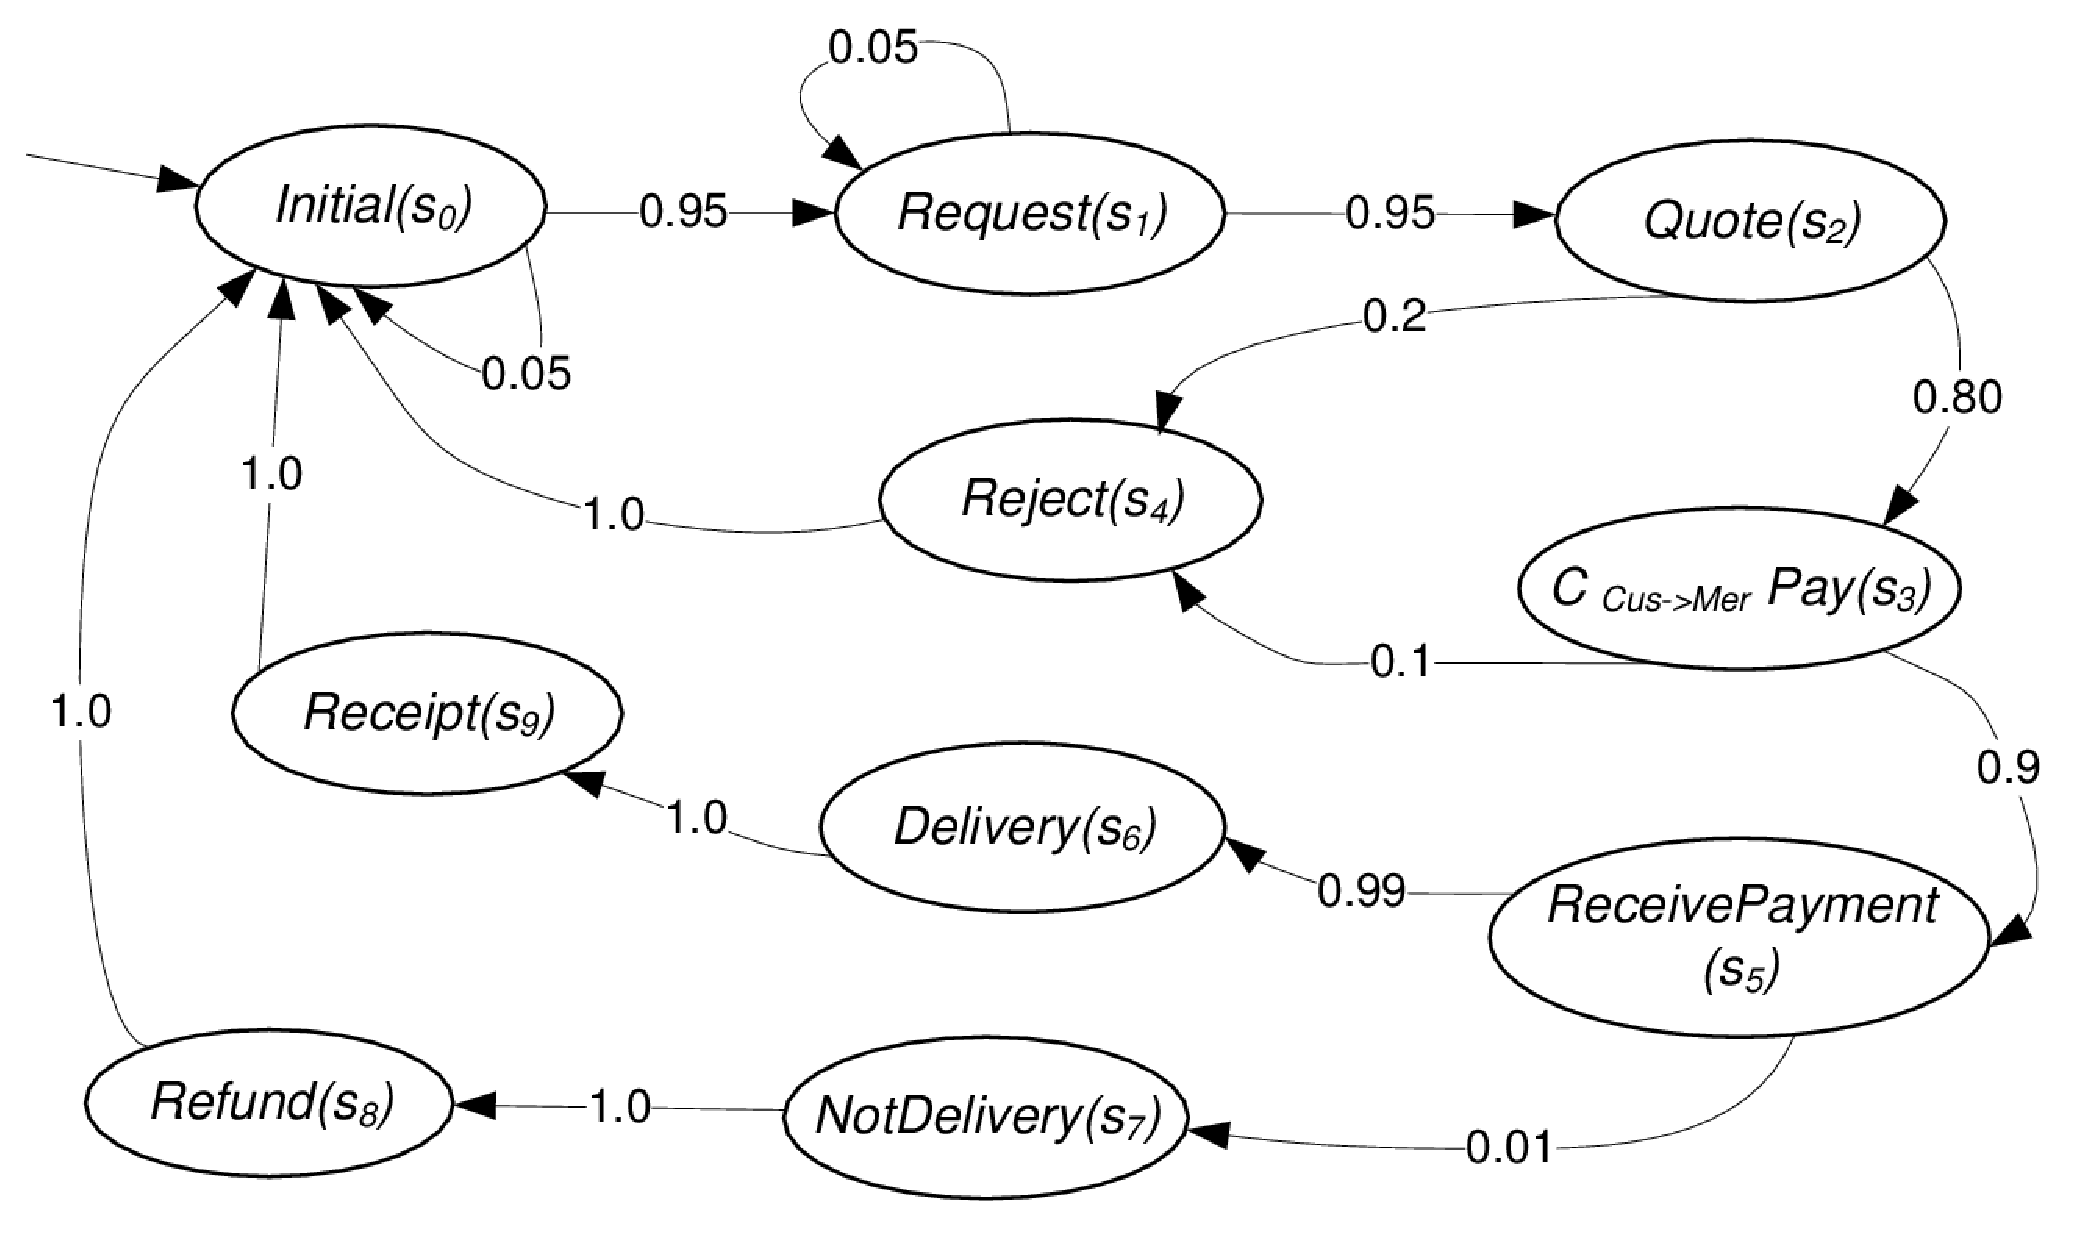
\includegraphics[width=14cm,height=8cm]{chap4/img/Netbill.eps}
\caption{The Modified NetBill protocol} \label{NetBill}
\end{center}
\end{figure}


With the PRISM modeling language, we translate every agent into a
\emph{module} and the entire MAS is defined as a system with \emph{agent modules} which are all synchronized.


To formalize the protocol, the scenario is encoded using the
probabilistic interpreted systems $\mathfrak{M_2}$ introduced earlier in Definition \ref{def:models-pctlkc}. Two basic modules, \emph{module
Mer1} and \emph{module Cur1} are defined according to their
probabilistic transitions. They represent the customer agent
\emph{Cus1} and the merchant agent \emph{Mer1} respectively. Other
agents can just refer to these two basic agents and use
\emph{module renaming} function to duplicate a module.

\subsection{NetBill Protocol Properties}

\begin{itemize}
\item \texttt{Safety property:} When designing a system, we may set a confidence interval to allow some mistakes for properties because it seems impossible for human beings not to make any mistake in the real world. For example, ``with 99\% chance, the system will not fail" instead of ``the system will never fail". In our protocol, one bad situation is when the customer $Cus1$ sends the payment to the merchant $Mer1$ without the merchant being aware of that. The following property can avoid this bad situation:

$\varphi_1 = \mathbb{P}_{= 1}$ $[\neg (Fu(C_{Cus1\rightarrow Mer1}Pay)
\wedge  (\neg K_{Mer1}Pay))]$.

This event is critical without any uncertainty. Therefore, we
set the probability to 1.
A similar formula is when the customer fulfills its commitments,
but it turns out that it is not aware of:

$\varphi_2 = \mathbb{P}_{= 1}$ $[\neg (Fu(C_{Cus1\rightarrow Mer1}Pay) \wedge  (\neg K_{Cus1}Pay))]$.

With 1\% tolerance for missing delivery, we can define the third
\emph{safety  property}  in our logic as follows:

$\varphi_3 = \mathbb{P}_{\geq 0.99}$ $[\neg (Fu(C_{Cus1 \rightarrow Mer1} Pay) \wedge
\neg (C_{Mer1\rightarrow Cur1} Delivery))]$.

\item \texttt{Liveness property:} Contrast to \emph{safety property}, a \emph{liveness property } means ``a good thing will eventually happen". For example, when the merchant commits to deliver the goods to the customer, it will eventually deliver them. This property is expressed as follows:

$\varphi_4 = \mathbb{P}_{\geq 0.99}(C_{Mer1 \rightarrow Cus1} Deliver\Rightarrow$
$\mathbb{P}_{\ge 0} [\text{F } Fu(C_{Mer1 \rightarrow Cus1} Deliver)]) $.

\item \texttt{Reachability property:} One good example for the reachability property for the NetBill protocol is that the merchant will eventually commit towards the customer to deliver the required goods, which should be reached from the initial state. This property can be expressed as follows:

$\varphi_5 = \mathbb{P}_{\geq 0}$ [F $C_{Mer1 \rightarrow Cus1} Deliver$]

\item \texttt{Quantitative properties:} One important usage for probabilistic model checking is to compute the actual probability of some behaviors of the system. We can calculate the probability for eventually the customer $Cus1$ commits to send the payment to the merchant $Mer1$ and eventually the customer fulfills the commitment:

$\varphi_6 = \mathbb{P}_{=?}$ [F $C_{Cur1 \rightarrow Mer1} Pay$]

$\varphi_7 = \mathbb{P}_{=?}$ [F $Fu(C_{Cur1 \rightarrow Mer1} Pay)$]

\end{itemize}




\subsection{Experimental Results}\label{sec:Experimental-results-cha4}

We verified several probabilistic epistemic and commitment
properties as well as combinations made up from both properties
for the NetBill protocol. The presented experiments were
performed on a Toshiba Port\'{e}g\'{e} computer
with 2.00 GHz Intel Core2 Duo T6400 processor and 3GB memory under
64-bit Windows Vista Operating System.


\begin{table} %[!htbp]
\centering \caption{Experimental results for NetBill protocol with
PRISM} \label{tab:result-cha4}
\begin{tabular}{|c|l|l|c|c|}
    \hline
    \texttt{Number}& \multicolumn{2}{c|}{\texttt{Model}} & \multicolumn{2}{c|}{\texttt{Construction}}\\
    \cline{2-5}
    \texttt{of Agents}  & \texttt{\#States} & \ \ \ \texttt{\#Transitions} & \texttt{Iterations} & \texttt{Time (sec)} \\
    \cline{1-5}
    \hline
    \hline
    2 &  19 & \ \ \ 39 & $7$ & $0.001$\\
    \hline
    $3$ &  $108$ & \ \ \ $432$ & $10$ & $0.008$\\
    \hline
    $4$ &  $979$ & \ \ \ $3.2*10^3$ & $13$ & $0.011$\\
    \hline
    $5$ &   $6.1*10^3$ & \ \ \ $24*10^3$ & $16$ & $0.024$\\
    \hline
    6 &  $38*10^3$ & \ \ \ $171*10^3$ & 19 & 0.028\\
    \hline
    7 &   $230*10^3$ & \ \ \ $1.1*10^6$ & 22 & 0.035\\
    \hline
    8 &   $1.4*10^6$ & \ \ \ $7.8*10^6$ & 25 & 0.049\\
    \hline
    9 &   $8.4*10^6$ & \ \ \ $52*10^6$ & 28 & 0.071\\
    \hline
    10 &  $50*10^6$ & \ \ \ $343*10^6$    & 31 & 0.097\\
    \hline
    15 & $392*10^9$ & \ \ \ $3.8*10^{12}$ & 46 & 0.498\\
    \hline
\end{tabular}
\end{table}

We have conducted 10 experiments for the protocol using up to 15
agents. The results are in Table \ref{tab:result-cha4}. Model
statistics data (number of states and number of transitions) and
model construction information (iteration and construction time)
are reported. The model statistics data reflect the state space,
while the construction information indicates the time for
converting the PRISM model into a symbolic model and iterations required to find the reachable states. We have noticed that the state space increases
exponentially as the number of agents increases. However, the time
needed for constructing the model increases polynomially as more
agents are added as shown in Figure \ref{Building the model-cha4}.


\begin{figure}%[!h]
\begin{center}
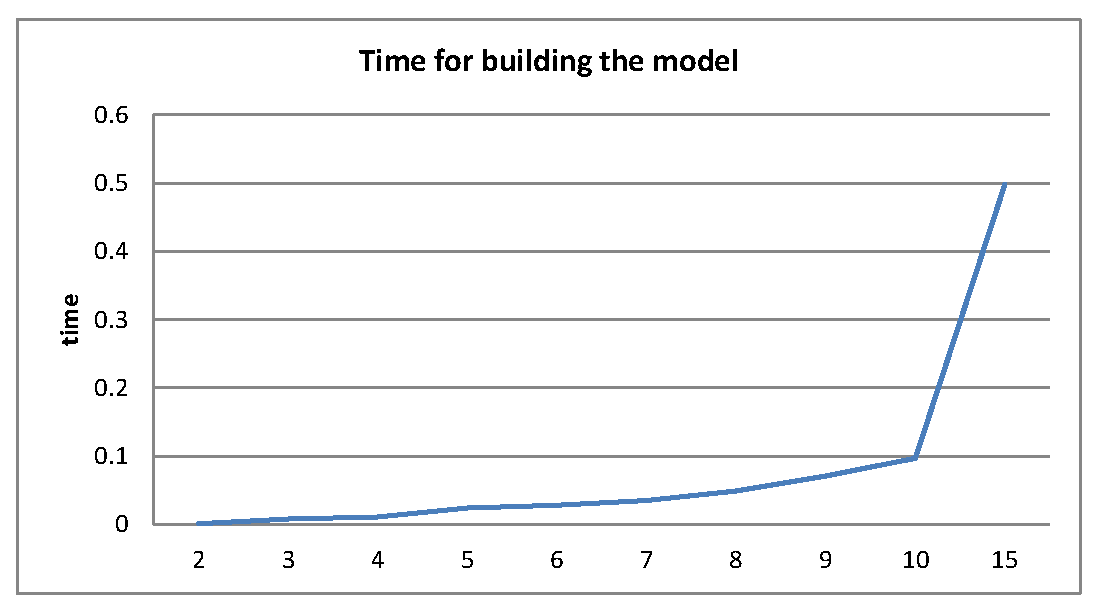
\includegraphics[width=10cm,height=6cm]{chap4/img/time-for-building-model.eps}
\caption{Model construction time for the NetBill protocol} \label{Building the model-cha4}
\end{center}
\end{figure}


We verified properties expressing some requirements of the NetBill
protocol that involve probabilistic knowledge and commitments. We
checked \emph{Safety, liveness,} and \emph{Reachability}
properties as discussed above. Table \ref{formulae-PRISM-results-cha4} shows the results of model checking the above desirable properties for the
probabilistic \emph{NetBill protocol} for a system that includes
one customer and one merchant.


\begin{table}%[H]
\centering \caption{Verifying some PCTL$^{kc}$ properties for the NetBill protocol in case of two agents} \label{formulae-PRISM-results-cha4}
\begin{tabular}{|c|c|c|}
\hline
\texttt{Formulae}    & \texttt{Results} & \texttt{Time for MC (sec)} \\
\hline\hline
$\varphi_1$                &True           &  0.001     \\
\hline
$\varphi_2$               &True           &  0.001     \\
\hline
$\varphi_3$                &True           & 0.008    \\
\hline
$\varphi_4$                &True          & 0.001   \\
\hline
$\varphi_5$                &True           &  0.008  \\
\hline
$\varphi_6$                &0.80           &  0.002  \\
\hline
$\varphi_7$                &0.72           &  0.001  \\
\hline

\end{tabular}
\end{table}

%%%%%%%%%%%%%%%%%%%%%%%%%%%%%%%%%%%%%%%%%%%%%%%%%%%%

\subsection{Discussion} \label{sec:discussion-cha4}

As we have seen in this chapter, a probabilistic logic for addressing the interaction between knowledge and social commitments in MASs was introduced. The described approach represents the first attempt in the literature to reason about and verify the interaction between the two concepts in the presence of uncertainty. However, from a consistency point of view, the logic we proposed seems to be inconsistent and suffers from some paradoxes like those identified in \cite{Al-Saqqar2014a}. The problem is that, one of the underlying logics of PCTL$^{kc}$, which is PCTLC \cite{Sultan2013}, is built using the social accessibility relation given in \cite{Bentahar2012,El-Menshawy2013a} which, in fact, over specifies and over constrains the concept of illocutionary communication.

In the next chapter, we see how we will overcome the aforementioned problem by extending a consisting logic of knowledge and commitment called CTLKC$^+$ \cite{Al-Saqqar2014a} by a probabilistic operator so that capturing and reasoning about the interaction between the concepts of knowledge and social commitments by means of a consistence probabilistic logic becomes possible. Moreover, the logic we introduce in Chapter \ref{cha:PCTLKC+} incorporates the concepts of group social commitments and group knowledge to the framework.



\section{Related Work} \label{sec:related-work-cha4}

The work presented in this chapter can be related to three perspectives
in the literature: probabilistic knowledge, probabilistic commitments,
and the interaction between the two aspects. In this section,
we review the relevant work with respect to probabilistic knowledge
and the interaction between probabilistic knowledge and probabilistic
commitments. However, for the relevant work on probabilistic
commitments, it has been discussed in Chapter \ref{cha:PCTLC}, Section \ref{sec:related-work-cha3}.

\subsection{Probabilistic Knowledge in MASs }

Delgado and Benevides in \cite{Delgado2009} defined a
probabilistic logic called K-PCTL which extends PCTL with an
epistemic operator for the knowledge.
For modeling their target systems, the authors proposed an
approach that represents each agent in the system as a DTMC with
synchronization actions. In their DTMC model, each state either
has a synchronized action with probability 1 or regular
probabilistic transitions. Having two different actions in a
single DTMC forced them to transform it into an MDP model. From
the semantics point of view, K-PCTL formulae are interpreted over
MDP models which are augmented with accessibility relations, so
that probabilities over paths can be defined. However, the
uncertainty of the knowledge cannot be measured as the
accessibility relations are not probabilistic. Our approach
differs from this one in four main points. First, our logic
adds two modalities on top of PCTL; one for the knowledge,
and one for the commitments and their fulfilments. Therefore, dimension of system's aspects that our logic can handle is larger than that of K-PCTL making it more expressive. Second, our logic permits the
probabilistic operator to precede each of the knowledge modality
and the social modality so that we can quantitatively reason about
the two aspects which again increases its expressive power. Third,
we model the target systems using probabilistic interpreted
systems. Forth, we propose a concrete model checking technique in
which we transform the problem of model checking our logic to the
problem of model checking an existing logic allowing us to re-use
the PRISM tool instead of just suggesting to extend it.

In \cite{Huang2011}, Huang and his colleagues extended the MCK
model checker \cite{Gammie2004} with subjective probability
relative to agent knowledge using interpreted partially observed
discrete-time Markov chain (PO-DTMC). PO-DTMC is based on partial
observations with assumption on synchronous with perfect recall.
To specify properties of probabilistic interpreted systems, the
authors use a logic that combines temporal and knowledge
modalities with a probabilistic operator. In their approach, the
set of accessible states is defined as states of a special agent,
called the environment, while the remaining agents observe the
environment and perform actions based on their observations. Then,
probabilistic knowledge is expressed by a rational linear
combination of every agents' probabilities in the system: every
agent has its own probability for each accessible state, which is
supposed to be known. Unlike this work, in our approach we do not
assume that accessibility transitions are probabilistic because
this information is not always accessible to agents and sometimes
hard to quantify. Instead, we compute the probabilistic knowledge
based on the number of accessible states as they are equally
accessible. Moreover, by re-using the exiting PRISM model checker,
we do not add a computational cost that is associated to extending
the existing version of it.


Wan et al. \cite{Wan2013} has also addressed the verification of
epistemic properties in agent environments  against the background
of participating parties. They propose PCTLK, a probabilistic,
epistemic,  branching-time logic which extends CTL with
probabilistic and epistemic modalities. To verify the proposed
logic, the authors introduced a reduction-based model checking
technique to translate the problem of model checking PCTLK into
the problem of model checking PCTL. Their reduction procedure
involves two processes. First, they transform the probabilistic
interpreted systems into an MDP which is transformed further to a
DTMC. Second, they translate each PCTLK formula into a
corresponding PCTL formula. To model check a PCTLK forumla, they
check its transformed PCTL formula over the DTMC model. They
demonstrated the applicability of their proposed verification
technique by applying it on a well known case study and
implementing it using the PRISM model checker. Our work is similar
to this work, except that we have a social modality in our
proposed logic for the commitments and their fulfilments which
makes it more expressive than PCTLK.


\subsection{The Interaction between Knowledge and Social Commitments}

Little work has been done towards the problem of capturing and verifying the interactions between knowledge and social commitments in MASs.

In \cite{Schmidt2004}, Schmidt and his colleagues investigated the
problem of formalizing the interaction between knowledge and
commitments within agent dynamic logic. Apparently, the commitment
adopted in this work is not a social commitment but rather an
internal commitment as the one presented by Castelfranchi in
\cite{Castelfranchi1995}. The term ``internal commitment'' refers to a commitment of an agent to itself \cite{Singh2008}. Using their proposed Agent Dynamic Logic (ADL), the authors were able to express some combinations between knowledge and commitments such as $Comm_i~(\alpha)\to K_i~Comm_i~(\alpha)$ which expresses that agent $i$ knows ($K_i$) about his
internal commitment ($Comm_i$) to perform the action $\alpha$.
However, from a communication perspective, the internal commitment
is neither communicative nor public because it is not created as
an agreement between two agents so that an agent can commit
towards the other to bring about a certain property. In contrast,
our work focuses primary on the notion of ``social commitment"
\cite{Singh2000} which has been used as a means of communication
between interacting agents in MASs. Unlike internal commitments,
which are private and concern a particular agent, social
commitments are public and observable engagements from one agent
to another agent or a group of agents to bring about something.  Furthermore, unlike \cite{Schmidt2004}, we study such an interaction ---between the two concepts--- in systems exhibiting probabilistic behaviors.

Al-Saqqar et al. \cite{Al-Saqqar2014a} have made the first attempt
towards studying the relationship between knowledge and
communicative social commitments from a logical perspective. In
particular, they combined a logic of knowledge (called CTLK
\cite{Lomuscio2007}) and a logic of commitments (called CTLC
\cite{Bentahar2012}) in a single tool called CTLKC. Having
analyzed some postulates with different combinations between the
two concepts expressed in CTLKC, the authors identified a set of
paradoxes that makes their combined logic inconsistent. To
overcome this problem, they mitigated the over-specification
problem that arises in the social accessibility relation given in
\cite{Bentahar2012,El-Menshawy2013a}. Intuitively and broadly
speaking, a social accessibility relation for two agents $i$ and
$j$ does exist between two global states $s_1$ and $s_2$ in the
system, if there is a communication channel between the local
states of $i$ and $j$ in the global states $s_1$ and $s_2$
respectively. Based on a new social accessibility relation, they
presented a new semantics for the commitment ($C_{i\rightarrow j}
\varphi$) and fulfilment ($Fu (C _{i\rightarrow j} \varphi)$)
operators, where $C_{i\rightarrow j} \varphi$ means that agent $i$
commits towards agent $j$ to bring about $\varphi$, and $Fu (C
_{i\rightarrow j} \varphi)$ expresses the fulfillment of such a
commitment. These changes have been integrated into a new
consistent logic named CTLKC$^+$. Having defined the new logic,
the authors have been successfully able to reason about various
combinations between knowledge $K_i \varphi$, which means that
agent $i$ knows $\varphi$, and social commitments as follows:

\begin{itemize}
\item $C_{i\rightarrow j} \varphi \Rightarrow K_i (C_{i\rightarrow
j} \varphi) $ where $i \neq j$.
\item $Fu (C _{i\rightarrow j} \varphi) \Rightarrow K _i \varphi$ where $i \neq j$.
\item $Fu (C _{i\rightarrow j} \varphi) \Rightarrow K_j \varphi$ where $i \neq j$.

\end{itemize}

Then, the authors introduced a reduction model checking technique
in which they transformed the problem of model checking their new
logic (CTLKC$^+$) into the problem of model checking an existing
logic called GCTL$^*$ \cite{Bhat2001}, and computed the complexity of the reduction technique. They used the automata-based model checker CWB-NC as the verification tool.

The verification of CTLKC$^+$ was further investigated in \cite{Al-Saqqar2014b}. The authors used a symbolic model checking technique based on reducing the problem of model checking CTLKC$^+$ into that of ARCTL. Then, they used the extended NuSMV to verify some given properties written in CTLKC$^+$. Their approach was carried out automatically using a JAVA transformation tool. This allowed them to overcome the scalability problem of automata-based model modeling checking techniques, which is a highly considerable problem in model checking real applications of multi-agent systems. The complexity analysis of the proposed reduction-based technique was also provided.

Unlike this work that tends to assume ideal behavior for MASs so it limits its application to reliable environments, ours considers the unreliable behavior of MASs. Therefore, we add a probabilistic modality to the logic to be able to reason about some desirable properties in the presence of uncertainty. Our proposal subsumes the one in \cite{Al-Saqqar2014a} because probability values range from 0 to 1 (when probability is equal to 1, the system becomes certain). Therefore, our framework outperforms this proposal in the sense that not only qualitative reasoning about the interaction between knowledge and commitments is achievable but also quantitative reasoning becomes possible.



\subsection{Comparison}

We compare our framework to the existing proposals by taking into
consideration five criteria: Knowledge, Commitments, Uncertainty,
Formalization, and Verification. Knowledge property shows whether
the approach addresses epistemic properties of the systems or not.
Commitments property indicates whether it addresses the social
commitments or not. Uncertainty reflects target systems whose
behavior is probabilistic. Formalization indicates the use of
formal logics, or formal methods in general. Finally, Verification
confirms the presentation of a formal verification technique to
verify the proposed approach. Table \ref{table:comparison} shows a
summary about the comparison between our framework and the
existing approaches based on the criteria described above.
We observe that our framework outperforms the related approaches as
it satisfies all the listed criteria.

\begin{table}
\centering \caption{Comparison between PCTL$^{kc}$ and the related work } \label{table:comparison}
\begin{tabular}{cccccc}
\hline
\texttt{Approach}       &\texttt{Knowledge} & \texttt{Commitment} & \texttt{Uncertainty}   & \texttt{Formal} & \texttt{Verification}\\
\hline
\cite{Witwicki2007,Witwicki2009}    &         &$\surd$   &$\surd$    &         &    \\
\cite{Huang2011}      &          &$\surd$   &$\surd$    &$\surd$  &$\surd$    \\
\cite{Delgado2009}     &$\surd$   &          &$\surd$    &$\surd$  &    \\
\cite{Wan2013}         &$\surd$   &          &$\surd$    &$\surd$  &$\surd$    \\
\cite{Al-Saqqar2014a}   &$\surd$   &$\surd$   &           &$\surd$  &$\surd$    \\
Our approach         &$\surd$   &$\surd$   &$\surd$    &$\surd$  &$\surd$    \\
\hline

\end{tabular}
\end{table}

To summarize, the advancement of our work over existing work lies in the expressiveness power of the proposed logic which allows autonomous agents in MASs to represent and verify the interaction between knowledge and social commitments in the face of uncertainty. Moreover, the new probabilistic interpreted systems introduced in this chapter helps MASs developers to have rich modeling with respect to knowledge and social commitments. That is, not only modeling knowledge and social commitments independently in the presence of uncertainty is possible, but also modeling the interaction between them has become possible by making use of our proposed probabilistic model.

%%%%%%%%%%%%%%%%%%%%%%%%%%%%%%%%%%%%%%%%%%%%%%%%%%%%%%%%%%%%%%%


\section{Summary}\label{sec:conclusion-cha4}

In this chapter, we presented a novel technique for specifying and evaluating the interaction between knowledge and social commitments in stochastic MASs. The proposed technique allows us, for the first time in the literature, to perform epistemic reasoning on social commitments in probabilistic MASs. This helps ensure agents' awareness about their commitments and the fulfillments of these commitments. In particular, we first developed a new version of interpreted systems that captures the probabilistic behavior of knowledge and commitments and accounts for the communication between interacting parties. Second, we defined a new logical framework that merges concepts of probabilistic knowledge and probabilistic commitments in a single logic called PCTL$^{kc}$, so that complex formulae including both modalities
can be expressed. Third, we introduced a new model checking
technique to formally verify the compliance of MASs against some
given properties expressed using the new logic. The proposed model
checking procedure is reduction-based, in which the problem of
model checking PCTL$^{kc}$ is transformed (by the use of some rules) into the problem of model checking an existing logic, namely PCTL. The key advantage of such a reduction is gaining the privilege to re-use a well
known model checker such as PRISM. The soundness of the proposed
reduction technique was provided. Moreover, we demonstrated the
effectiveness of the proposed framework by applying it to the
NetBill protocol, a concrete case study from e-business domain.
The results have initially confirmed the expressive
capabilities of PCTL$^{kc}$ in handling the
interaction between knowledge and social commitments in
probabilistic settings. Moreover, the scalability of the proposed model
checking technique was evaluated and models having up to $4
\times 10^{11}$ states can be effectively verified.

In the next chapter, we refine and extend the approach presented for the interaction between individual knowledge and commitments to accommodate  group knowledge and group commitments as well.
